\documentclass[10pt]{article}

\usepackage[utf8]{inputenc}
\usepackage[spanish]{babel}
\decimalpoint
\usepackage{amsmath, amssymb}
\usepackage{xcolor}
\usepackage{geometry}
\geometry{letterpaper, margin=1in}
\usepackage{graphicx}
\usepackage{float}
\usepackage{array}
\usepackage{booktabs}
\usepackage{colortbl}
\usepackage{caption}
\usepackage{tocloft}

\usepackage[colorlinks=true, linkcolor=black, urlcolor=black, citecolor=black]{hyperref}
%%%%%%%%%%%%%%%%%%%%%%%%%%%%%%%%%%%%%%%%%%%%%%%%%%%%%%%%%%%%%%%%%%%%%%%%%%%%%%%%%%%%%%%%%%%%%%%%%%%%%%%%%%%%%%
%%%%%%%%%%%%%%%%%%%%%%%%%%%%%%%%%%%%%%%%%%%%%%%%%%%%%%%%%%%%%%%%%%%%%%%%%%%%%%%%%%%%%%%%%%%%%%%%%%%%%%%%%%%%%%
\title{Universidad Panamericana \\ Maestría en Ciencia de Datos \\ Datos Masivos \\ 
    \vspace{0.5cm} Proyecto Final: \textit{Monitoreo Inteligente de Tráfico Marítimo con Big Data AIS}}
\author{Enrique Ulises Báez Gómez Tagle, Luis Alejandro Guillén Alvarez}
\date{\today}
%%%%%%%%%%%%%%%%%%%%%%%%%%%%%%%%%%%%%%%%%%%%%%%%%%%%%%%%%%%%%%%%%%%%%%%%%%%%%%%%%%%%%%%%%%%%%%%%%%%%%%%%%%%%%%
%%%%%%%%%%%%%%%%%%%%%%%%%%%%%%%%%%%%%%%%%%%%%%%%%%%%%%%%%%%%%%%%%%%%%%%%%%%%%%%%%%%%%%%%%%%%%%%%%%%%%%%%%%%%%%
%%%%%%%%%%%%%%%%%%%%%%%%%%%%%%%%%%%%%%%%%%%%%%%%%%%%%%%%%%%%%%%%%%%%%%%%%%%%%%%%%%%%%%%%%%%%%%%%%%%%%%%%%%%%%%%%%%%%%%%%%%%%%%%%%%%%%%%%%%%%%%%%%%%%%%%%%%%%%%%%%%%%%%%%%%%%%%%%%%%%%%%%%%%%%%
%%%%%%%%%%%%%%%%%%%%%%%%%%%%%%%%%%%%%%%%%%%%%%%%%%%%%%%%%%%%%%%%%%%%%%%%%%%%%%%%%%%%%%%%%%%%%%%%%%%%%%%%%%%%%%%%%%%%%%%%%%%%%%%%%%%%%%%%%%%%%%%%%%%%%%%%%%%%%%%%%%%%%%%%%%%%%%%%%%%%%%%%%%%%%%
\begin{document}

\maketitle

\tableofcontents

\newpage

%%%%%%%%%%%%%%%%%%%%%%%%%%%%%%%%%%%%%%%%%%%%%%%%%%%%%%%%%%%%%%%%%%%%%%%%%%%%%%%%%%%%%%%%%%%%%%%%%%%%%%%%%%%%%%%%%%%%%%%%%%%%%%%%%%%%%%%%%%%%%%%%%%%%%%%%%%%%%%%%%%%%%%%%%%%%%%%%%%%%%%%%%%%%%%
%%%%%%%%%%%%%%%%%%%%%%%%%%%%%%%%%%%%%%%%%%%%%%%%%%%%%%%%%%%%%%%%%%%%%%%%%%%%%%%%%%%%%%%%%%%%%%%%%%%%%%%%%%%%%%%%%%%%%%%%%%%%%%%%%%%%%%%%%%%%%%%%%%%%%%%%%%%%%%%%%%%%%%%%%%%%%%%%%%%%%%%%%%%%%%
\section{Resumen ejecutivo}
\subsection{Introducción} 

El tráfico marítimo global genera millones de registros de posicionamiento a través del Sistema de Identificación Automática (AIS), que transmite automáticamente la identidad, posición, velocidad y otros datos de los buques. Originalmente implementado para mejorar la seguridad de la navegación, hoy es crucial para la gestión del tráfico marítimo, la conciencia del entorno y operaciones de búsqueda y rescate.

Este proyecto propone aprovechar Big Data y aprendizaje automático (ML) para analizar una base de datos masiva de mensajes AIS y ofrecer una solución innovadora a la pregunta: \textbf{¿Cómo detectar y entender comportamientos anómalos en el tráfico marítimo para mejorar la seguridad y la eficiencia?}

Responder esta pregunta implica analizar patrones normales de navegación y descubrir desviaciones significativas. En esencia:
\begin{itemize}
    \item \textbf{¿Qué estamos haciendo?} Diseñamos un sistema de análisis que procesa grandes volúmenes de datos AIS para identificar anomalías en el comportamiento de los buques (posiciones fuera de lugar, velocidades inusuales, maniobras erráticas, etc.) y extraer patrones útiles sobre la operación de diferentes tipos de embarcaciones.
    \item \textbf{¿Para qué lo hacemos?} Para mejorar la seguridad marítima, la gestión del tráfico y la toma de decisiones, ofreciendo alertas tempranas de potenciales riesgos (colisiones, actividades ilícitas o fallos) y conocimiento profundo a autoridades y empresas navieras.
    \item \textbf{¿Cómo lo hacemos?} Empleando herramientas de Big Data de la Suite de Google Cloud (Storage + DataProc + BigQuery) para procesar datos geoespaciales masivos en en poco tiempo, complementado con modelos de ML que aprenden patrones habituales y detectan comportamientos que se apartan de lo normal.
    \item \textbf{¿A quién beneficia?} A organismos de seguridad marítima (marinas, guardacostas), a empresas navieras optimizando rutas y monitoreo de flotas, a aseguradoras evaluando riesgos operativos e incluso a investigadores del medio marino en estudios ecológicos.
\end{itemize}

Finalmente, los resultados se integraron en un \textit{dashboard} interactivo con visualizaciones (mapas geográficos, gráficos de tendencias y rankings) que facilitan la interpretación y la toma de decisiones.
%%%%%%%%%%%%%%%%%%%%%%%%%%%%%%%%%%%%%%%%%%%%%%%%%%%%%%%%%%%%%%%%%%%%%%%%%%%%%%%%%%%%%%%%%%%%%%%%%%%%%%%%%%%%%%%%%%%%%%%%%%%%%%%%%%%%%%%%%%%%%%%%%%%%%%%%%%%%%%%%%%%%%%%%%%%%%%%%%%%%%%%%%%%%%%
%%%%%%%%%%%%%%%%%%%%%%%%%%%%%%%%%%%%%%%%%%%%%%%%%%%%%%%%%%%%%%%%%%%%%%%%%%%%%%%%%%%%%%%%%%%%%%%%%%%%%%%%%%%%%%%%%%%%%%%%%%%%%%%%%%%%%%%%%%%%%%%%%%%%%%%%%%%%%%%%%%%%%%%%%%%%%%%%%%%%%%%%%%%%%%
\section{Visión general del desarrollo} 
\subsection{Solución Actual / visión general} % TODO GUILLÉN: FALTA AÑADIR PARTE DE ML tanto descripción como diagrama

La solución actual se implementa de extremo a extremo sobre la nube de Google Cloud. El flujo completo es el siguiente:

\begin{itemize}
    \item Una máquina virtual en Google Compute Engine se encarga de \textbf{scrapear los datos AIS} y cargarlos en Google Cloud Storage. 
    \item En Cloud Storage se organizan dos capas diferenciadas: \textit{raw} y \textit{curated}, con prefijos de carpeta y particiones por mes (\texttt{YYYY-MM=}).
    \item Un clúster de Google Cloud DataProc (perfil \emph{high-memory}; véase Sección~\ref{sec:cluster}) ejecuta dos jobs, habilitando procesamientos por series de meses con menos derrames a disco y menor tiempo total:
    \begin{itemize}
        \item Job \textbf{raw}: descomprime los archivos obtenidos y organiza los datos en particiones por año y mes, y finalmente los guarda en formato Parquet en Google Cloud Storage.
        \item Job \textbf{curated}: lee la capa cruda, aplica transformaciones iniciales y genera la capa refinada lista para análisis.
    \end{itemize}
    \item Una Cloud Function crea el \textbf{dataset y la tabla en BigQuery}, cargando la información desde la capa curated.
    \item En BigQuery se centraliza la explotación de datos mediante consultas SQL optimizadas, generando los datasets finales que alimentan las visualizaciones.
    \item El \textbf{dashboard de Streamlit}, desplegado en la misma VM, consume los resultados de BigQuery y presenta mapas, gráficos de tendencias y rankings de manera interactiva.
\end{itemize}

\vspace{0.5cm}
\begin{figure}[H]
    \centering
    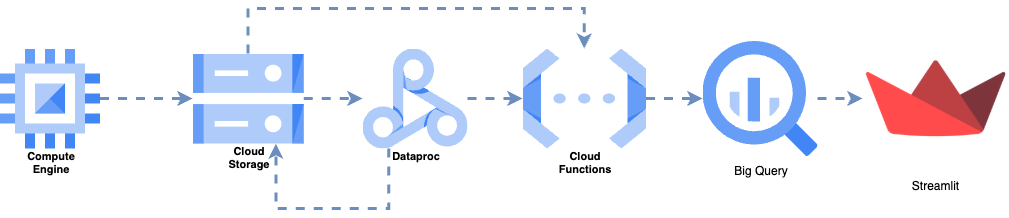
\includegraphics[width=\textwidth]{figures/arch/ArchitectureDiagram.png}
    \caption{Arquitectura actual de la solución: flujo end-to-end en Google Cloud.}
\end{figure}
\vspace{0.1cm}
%%%%%%%%%%%%%%%%%%%%%%%%%%%%%%%%%%%%%%%%%%%%%%%%%%%%%%%%%%%%%%%%%%%%%%%%%%%%%%%%%%%%%%%%%%%%%%%%%%%%%%%%%%%%%%%%%%%%%%%%%%%%%%%%%%%%%%%%%%%%%%%%%%%%%%%%%%%%%%%%%%%%%%%%%%%%%%%%%%%%%%%%%%%%%%
%%%%%%%%%%%%%%%%%%%%%%%%%%%%%%%%%%%%%%%%%%%%%%%%%%%%%%%%%%%%%%%%%%%%%%%%%%%%%%%%%%%%%%%%%%%%%%%%%%%%%%%%%%%%%%%%%%%%%%%%%%%%%%%%%%%%%%%%%%%%%%%%%%%%%%%%%%%%%%%%%%%%%%%%%%%%%%%%%%%%%%%%%%%%%%
\subsection{Limitaciones actuales de la solución}
\label{subsec:limitaciones-solucion}

\begin{itemize}
  \item \textbf{Sin orquestación event-driven.} Los disparadores son manuales o programados; la activación automática por eventos de GCS/Pub\,\/Sub o Workflows aún no está implementada. Migrar a un esquema event-driven reduciría intervención manual y tiempos de ciclo.
  \item \textbf{No tiempo real.} El pipeline es \textit{batch}; no hay ingesta en streaming ni SLA de latencia. El dashboard refleja cortes al cierre de cada corrida.
  \item \textbf{Evolución de esquema limitada.} La Cloud Function crea tablas y puede autodetectar esquema, pero no hay un proceso formal de migraciones/versionado ni \textit{backfills} automatizados.
  \item \textbf{Pruebas y monitoreo.} Podrían generarse alertas proactivas (Cloud Monitoring/Error Reporting) ante fallas o derivas.
\end{itemize}

%%%%%%%%%%%%%%%%%%%%%%%%%%%%%%%%%%%%%%%%%%%%%%%%%%%%%%%%%%%%%%%%%%%%%%%%%%%%%%%%%%%%%%%%%%%%%%%%%%%%%%%%%%%%%%%%%%%%%%%%%%%%%%%%%%%%%%%%%%%%%%%%%%%%%%%%%%%%%%%%%%%%%%%%%%%%%%%%%%%%%%%%%%%%%%
%%%%%%%%%%%%%%%%%%%%%%%%%%%%%%%%%%%%%%%%%%%%%%%%%%%%%%%%%%%%%%%%%%%%%%%%%%%%%%%%%%%%%%%%%%%%%%%%%%%%%%%%%%%%%%%%%%%%%%%%%%%%%%%%%%%%%%%%%%%%%%%%%%%%%%%%%%%%%%%%%%%%%%%%%%%%%%%%%%%%%%%%%%%%%%
\subsection{Propósito, uso y alcance de la herramienta}
\noindent\textbf{Propósito general.} La herramienta tiene como propósito transformar los mensajes AIS masivos en \textit{inteligencia operable} para seguridad y gestión del tráfico marítimo. Provee un flujo reproducible de ingesta, depuración, análisis y detección de anomalías que permita identificar comportamientos de riesgo (velocidades inusuales, cambios de rumbo bruscos, calados atípicos, derivas de patrones por zona/tipo de buque) y entregar hallazgos mediante un \textit{dashboard} interactivo.

\vspace{0.2cm}
\noindent\textbf{Objetivos específicos.}
\begin{itemize}
  \item \textbf{Monitoreo descriptivo y exploratorio:} caracterizar el comportamiento típico por tipo de embarcación (\textit{VesselTypeName}), zona (\texttt{geohash9}) y periodo (hora/día), incluyendo estados de navegación y métricas de velocidad/rumbo.
  \item \textbf{Detección temprana de anomalías:} señalar observaciones que se desvían significativamente de los patrones normales (p.ej., \emph{z-scores} de calado, picos de velocidad, virajes abruptos) y, a nivel temporal, detectar valores atípicos con modelos ARIMA\_PLUS en BigQuery ML.
  \item \textbf{Soporte a decisiones:} priorizar buques, zonas y ventanas temporales que requieren atención, entregando listas y visualizaciones accionables para autoridades y operadores.
  \item \textbf{Escalabilidad y reproducibilidad:} estandarizar el pipeline en Google Cloud (Storage, DataProc, BigQuery, Cloud Functions) para procesar volúmenes elevados con costos y tiempos controlados.
\end{itemize}

\vspace{0.2cm}
\noindent\textbf{Usuarios objetivo y decisiones habilitadas.}
\begin{itemize}
  \item \textbf{Autoridades marítimas/guardacostas:} focalización de patrullajes y verificación de eventos inusuales por zona-tiempo-buque.
  \item \textbf{Navieras y operadores de flota:} supervisión de cumplimiento operativo, eficiencia de rutas y detección de riesgos operativos.
  \item \textbf{Aseguradoras y analistas de riesgo:} evidencia cuantitativa para evaluación de siniestralidad y \textit{pricing} técnico.
  \item \textbf{Investigación/medio marino:} análisis de patrones de movilidad y su interacción con áreas sensibles.
\end{itemize}

\vspace{0.2cm}
\noindent\textbf{Casos de uso cubiertos en el \textit{dashboard}.} Cada módulo se respalda con consultas SQL parametrizables en BigQuery:
\begin{itemize}
  \item \textbf{Calado anómalo} (\emph{per buque y tipo}): cálculo de \emph{z-score} sobre el calado medio por MMSI dentro de su categoría, para resaltar posibles inconsistencias operativas o de reporte.
  \item \textbf{Cambios de dirección bruscos} (\emph{virajes}): detección de deltas de rumbo (\texttt{COG}) sobre series temporales por MMSI, agregados por \texttt{geohash9}, con umbrales configurables de severidad.
  \item \textbf{Velocidades inusuales}: comparación del \textit{máximo} de \texttt{SOG} contra percentiles de referencia por buque/tipo para evidenciar excesos.
  \item \textbf{Variabilidad de velocidad y rumbo}: \texttt{STDDEV} y \texttt{AVG} de \texttt{SOG}/\texttt{COG} por tipo de embarcación como indicador de estabilidad operacional.
  \item \textbf{Correlaciones estructurales}: relaciones \texttt{Length–Width} (eslora–manga) por clase de buque y correlaciones entre métricas operativas (p.ej., \texttt{SOG} vs. \texttt{COG}) con filtros de tamaño muestral.
  \item \textbf{Resumen de estados de navegación}: conteos, embarcaciones únicas y promedios (\texttt{SOG}, calado) por \texttt{NavStatusName}.
  \item \textbf{Patrones semanales}: velocidad promedio y estado de navegación más frecuente por día de la semana y tipo de buque.
  \item \textbf{Ubicación y trazas recientes} (\texttt{geohash9}): listados y mapas de últimas posiciones por filtros de fecha, tipo de buque o MMSI.
  \item \textbf{Detección de anomalías temporales con ML}: entrenamiento y consulta de modelos \texttt{ARIMA\_PLUS} por serie (\texttt{geohash9}, \texttt{VesselTypeName} o \texttt{MMSI}) para marcar valores atípicos con umbrales de probabilidad ajustables.
\end{itemize}

\vspace{0.2cm}
\noindent\textbf{Entradas, procesamiento y salidas.}
\begin{itemize}
  \item \textbf{Entradas:} archivos AIS 2024 (NOAA) descargados y versionados en GCS (\textit{raw}/\textit{curated}), con partición temporal.
  \item \textbf{Procesamiento:} DataProc (Spark) para descompresión, partición y normalización; BigQuery para \textit{modelado analítico}, agregaciones y ML.
  \item \textbf{Salidas:} tablas refinadas y \textit{views} listas para consumo, modelos ML en \texttt{dataset} dedicado y un \textit{dashboard} Streamlit con mapas, tendencias y rankings exportables.
\end{itemize}

\vspace{0.2cm}
\newpage
\noindent\textbf{Alcance (in/out-of-scope).}
\begin{itemize}
  \item \textbf{Incluye:} análisis \textit{batch}, filtros por ventana temporal y región, métricas descriptivas, detección de anomalías no supervisada (estadística y ARIMA\_PLUS), visualizaciones interactivas y \textit{ranking} de eventos/buques.
  \item \textbf{No incluye (versión actual):} ingesta \textit{streaming} tiempo real, orquestación \textit{event-driven}, \textit{backfills} automáticos de esquemas, clasificación supervisada de ilícitos, reconstrucción de trayectorias de alta fidelidad ni generación de alertas operativas en caliente.
\end{itemize}

\vspace{0.2cm}
\noindent\textbf{Supuestos y restricciones.}
\begin{itemize}
  \item Calidad y cobertura del AIS dependen de la fuente; pueden existir vacíos, duplicados o reportes erróneos.
  \item El desempeño está condicionado por la configuración del clúster DataProc y los límites/cuotas de BigQuery; se privilegia costo-eficiencia sobre latencia.
  \item La zonificación espacial usa \texttt{geohash9} como índice geoespacial operacional.
\end{itemize}

%%%%%%%%%%%%%%%%%%%%%%%%%%%%%%%%%%%%%%%%%%%%%%%%%%%%%%%%%%%%%%%%%%%%%%%%%%%%%%%%%%%%%%%%%%%%%%%%%%%%%%%%%%%%%%%%%%%%%%%%%%%%%%%%%%%%%%%%%%%%%%%%%%%%%%%%%%%%%%%%%%%%%%%%%%%%%%%%%%%%%%%%%%%%%%
\section{Revisión y uso de datos}
\subsection{Orígenes y control de datos}

Los datos utilizados provienen del portal oficial de la NOAA (\url{https://coast.noaa.gov/htdata/CMSP/AISDataHandler/2024/index.html}), el cual publica archivos comprimidos (.zip) con los mensajes AIS recolectados a lo largo del año 2024. 
Para garantizar la trazabilidad y el control de los datos, se desarrolló un script en Python (\texttt{scrapper.py}) que automatiza la descarga de todos los archivos disponibles, verificando duplicados mediante el tamaño de los ficheros y evitando descargas innecesarias. 
De esta manera se asegura que la totalidad de los datos originales publicados por la NOAA sean capturados sin alteración.

%%%%%%%%%%%%%%%%%%%%%%%%%%%%%%%%%%%%%%%%%%%%%%%%%%%%%%%%%%%%%%%%%%%%%%%%%%%%%%%%%%%%%%%%%%%%%%%%%%%%%%%%%%%%%%%%%%%%%%%%%%%%%%%%%%%%%%%%%%%%%%%%%%%%%%%%%%%%%%%%%%%%%%%%%%%%%%%%%%%%%%%%%%%%%%
\subsection{Preparación de datos}
En esta sección se describe el \textbf{qué} produce la preparación de datos (entradas, salidas y \emph{esquema}); la orquestación y operación del pipeline (el \textbf{cómo}) se documenta en la Sección~\ref{sec:metodologia}.

La preparación de los datos comienza en una máquina virtual de Google Compute Engine, donde se ejecuta el script de \textit{scraping}. Este proceso descarga en paralelo (con \textit{threads}) los archivos \texttt{.zip} hacia un directorio local (\texttt{ais\_2024}) y posteriormente los traslada a Google Cloud Storage en la capa \textbf{raw}.\\

Dado el objetivo de tener un conjunto uniforme, trazable y listo para análisis, con: (i) esquema estandarizado, (ii) claves y derivadas temporales, (iii) coordenadas y velocidades normalizadas, y (iv) datos particionados por \texttt{ym} (AAAA-MM).

\paragraph{Entradas $\rightarrow$ salidas por etapa y la salida de cada una.}
\begin{enumerate}
  \item \textbf{RAW INGESTION}: entrada = lotes \texttt{.zip} de NOAA; salida = archivos Parquet en \textbf{raw} \emph{particionados por \texttt{ym}}, con trazabilidad mínima (archivo fuente y timestamp de ingesta).
  \item \textbf{CURATED TRANSFORMATIONS}: entrada = \textbf{raw}; salida = capa \textbf{curated} con tipos normalizados, derivados temporales y desduplicación por \texttt{MMSI+BaseDateTime}. Las reglas de limpieza y validaciones se detallan en la Sección~\ref{sec:cleaning}.
\end{enumerate}

\paragraph{Modelo de datos de la capa \textit{curated}.}
El Cuadro~\ref{tab:curated_schema} presenta los campos principales que expone la capa analítica.

\begin{table}[H]
  \centering
  \caption{Esquema de la capa \textit{curated}.}
  \label{tab:curated_schema}
  \scriptsize
  \begin{tabular}{@{}llp{8cm}@{}}
  \toprule
  Campo & Tipo & Descripción \\
  \midrule
  NavStatusInt & INTEGER & Representación entera del estado de navegación del buque. \\
  MMSI & STRING & Número de Identidad del Servicio Móvil Marítimo del buque. \\
  BaseDateTime & TIMESTAMP & Marca temporal que indica la fecha y hora del mensaje AIS. \\
  LAT & FLOAT & Latitud de la posición del buque. \\
  LON & FLOAT & Longitud de la posición del buque. \\
  SOG & FLOAT & Velocidad sobre el fondo del buque en nudos. \\
  COG & FLOAT & Rumbo sobre el fondo del buque en grados. \\
  Heading & FLOAT & Rumbo de la proa del buque en grados. \\
  VesselName & STRING & Nombre del buque. \\
  IMO & STRING & Número de la Organización Marítima Internacional del buque. \\
  CallSign & STRING & Indicativo de llamada por radio del buque. \\
  VesselType & STRING & Tipo de buque. \\
  Status & STRING & Estado del buque. \\
  Length & FLOAT & Eslora del buque. \\
  Width & FLOAT & Manga del buque. \\
  Draft & FLOAT & Calado del buque. \\
  Cargo & STRING & Tipo de carga que transporta el buque. \\
  TransceiverClass & STRING & Clase del transpondedor AIS. \\
  \_source\_file & STRING & Nombre del archivo fuente desde el cual se ingirieron los datos. \\
  \_ingest\_ts & TIMESTAMP & Marca temporal que indica cuándo se ingirieron los datos en la tabla. \\
  ymd & STRING & Fecha en formato año-mes-día. \\
  VesselTypeInt & INTEGER & Representación entera del tipo de buque. \\
  VesselTypeCode & STRING & Código que representa el tipo de buque. \\
  VesselTypeName & STRING & Nombre del tipo de buque. \\
  VesselTypeClass & STRING & Clasificación del tipo de buque. \\
  NavStatusName & STRING & Nombre del estado de navegación del buque. \\
  date & DATE & Fecha en que se registró el mensaje AIS. \\
  hour & INTEGER & Hora del día en que se registró el mensaje AIS. \\
  dow & STRING & Día de la semana en que se registró el mensaje AIS. \\
  week & INTEGER & Semana del año en que se registró el mensaje AIS. \\
  month & INTEGER & Mes en que se registró el mensaje AIS. \\
  quarter & INTEGER & Trimestre del año en que se registró el mensaje AIS. \\
  SOG\_ms & FLOAT & Velocidad sobre el fondo del buque en metros por segundo. \\
  geohash9 & STRING & Representación geohash de la posición del buque con precisión de 9 caracteres. \\
  \bottomrule
  \end{tabular}
\end{table}

Una vez procesado, el resultado de este pipeline se publica en BigQuery como tabla particionada por \texttt{ym}, optimizada para consulta y consumo por el \textit{dashboard}. Los detalles de automatización de creación/carga (Cloud Function, idempotencia y autodetección de esquema) se abordan en la Sección~\ref{sec:metodologia}.
%%%%%%%%%%%%%%%%%%%%%%%%%%%%%%%%%%%%%%%%%%%%%%%%%%%%%%%%%%%%%%%%%%%%%%%%%%%%%%%%%%%%%%%%%%%%%%%%%%%%%%%%%%%%%%%%%%%%%%%%%%%%%%%%%%%%%%%%%%%%%%%%%%%%%%%%%%%%%%%%%%%%%%%%%%%%%%%%%%%%%%%%%%%%%%
\subsection{Limpieza y tratamiento de datos} 
\label{sec:cleaning}

En esta sección se describen de manera detallada las transformaciones y criterios aplicados para convertir los datos AIS en una capa \textbf{curated} funcional para el análisis. Se listan los pasos con su \emph{porqué} operativo o estadístico.

\paragraph{Normalizaciones y tipos.}
\begin{itemize}
  \item \textbf{Casteo y estandarización}: se convierten columnas numéricas a tipos adecuados (\texttt{double}/\texttt{int}) y se normalizan textos (\texttt{trim}, mayúsculas controladas) para evitar variabilidad en joins/agrupaciones.
  \item \textbf{Timestamps en UTC}: \texttt{BaseDateTime} se parsea a tipo timestamp con zona UTC para análisis temporales coherentes; sobre esta base se derivan \texttt{date}, \texttt{hour}, \texttt{week}, \texttt{month}, \texttt{quarter} y una columna \texttt{ym} (AAAA-MM) para particionado.
\end{itemize}

\paragraph{Coordenadas y límites físicos.}
\begin{itemize}
  \item \textbf{LAT/LON válidos}: se recortan latitudes al rango [-90, 90] y longitudes se \emph{envuelven} a [-180, 180] (corrigiendo valores fuera de dominio por errores/reporte). Se descartan registros con coordenadas nulas tras la corrección.
  \item \textbf{Redondeo razonable}: se redondean LAT/LON a 5 decimales para homogenizar precisión sin perder resolución náutica relevante.
\end{itemize}

\paragraph{Velocidad, rumbos y estados.}
\begin{itemize}
  \item \textbf{SOG (Speed Over Ground)}: se acota a [0, 70] nudos para eliminar outliers físicos/telemetría corrupta; adicionalmente se calcula \texttt{SOG\_ms} en m/s para modelos.
  \item \textbf{COG/Heading}: se normaliza módulo 360°. El valor \texttt{Heading=511} (no disponible) se marca como nulo para evitar sesgos en métricas de rumbo.
  \item \textbf{NavStatus}: se genera \texttt{NavStatusInt} a partir de \texttt{Status} y se une contra un catálogo para \texttt{NavStatusName}; códigos fuera de 0–15 se etiquetan como \textit{Unknown} y faltantes como \textit{Not reported}.
\end{itemize}

\paragraph{Dimensiones y calado.}
\begin{itemize}
  \item \textbf{Length/Width}: se acotan a rangos plausibles (1–450 m y 1–70 m, respectivamente) para descartar errores de orden de magnitud.
  \item \textbf{Draft}: se limita a [0, 25] m; valores negativos o excesivos suelen provenir de carga mal reportada o errores de parsing.
\end{itemize}

\paragraph{Identificadores y texto.}
\begin{itemize}
  \item \textbf{MMSI}: se extrae la porción numérica válida (1–9 dígitos) y se rellena a 9 con ceros a la izquierda para formato consistente.
  \item \textbf{IMO/CallSign/VesselName}: se normalizan espacios y caracteres no alfanuméricos; se limpian IMOs genéricos (p.ej., \texttt{IMO0000000}, \texttt{0}, vacío) para evitar falsas uniones.
\end{itemize}

\paragraph{Clasificación de tipo de buque.}
\begin{itemize}
  \item \textbf{VesselType}: se derivan \texttt{VesselTypeInt}, \texttt{VesselTypeName} (mediante mapa IMO) y \texttt{VesselTypeClass} (WIG, Cargo, Tanker, Passenger, etc.). Esto permite comparar métricas por clase homogénea y soportar reglas dependientes del tipo.
\end{itemize}

\paragraph{Enriquecimiento geoespacial.}
\begin{itemize}
  \item \textbf{Geohash9}: se calcula un \texttt{geohash9} distribuido (UDF con \texttt{pygeohash}) para agregación espacial eficiente y enlaces a capas geográficas (vallas, puertos, TSS) en análisis posteriores.
\end{itemize}

\paragraph{Calidad e idempotencia.}
\begin{itemize}
  \item \textbf{Desduplicación}: se eliminan duplicados por clave compuesta \texttt{(MMSI, BaseDateTime)} para asegurar series temporales limpias por embarcación.
  \item \textbf{Validación de conteos}: en \textit{raw}, se comparan conteos diarios (CSV vs Parquet) y se aborta si no coinciden; en \textit{curated}, se escriben marcadores de éxito por partición (\texttt{\_markers/ym=.../\_SUCCESS}) para reanudación y ejecución incremental sin sobrescribir trabajo correcto.
\end{itemize}
%%%%%%%%%%%%%%%%%%%%%%%%%%%%%%%%%%%%%%%%%%%%%%%%%%%%%%%%%%%%%%%%%%%%%%%%%%%%%%%%%%%%%%%%%%%%%%%%%%%%%%%%%%%%%%%%%%%%%%%%%%%%%%%%%%%%%%%%%%%%%%%%%%%%%%%%%%%%%%%%%%%%%%%%%%%%%%%%%%%%%%%%%%%%%%
\subsection{Limitaciones de los datos}
\label{sec:limitaciones-datos}

\vspace{0.2cm}
\noindent\textbf{Limitaciones de origen y cobertura.}
\begin{itemize}
  \item \textbf{Cobertura heterogénea:} la recepción varía por densidad de estaciones y condiciones atmosféricas; en zonas costeras y puertos existe mejor cobertura que en mar abierto.
  \item \textbf{Congestión y pérdida de mensajes:} en áreas de alto tráfico se producen colisiones de ranuras/transmisiones y \emph{dropouts}; los conteos absolutos pueden estar subestimados.
  \item \textbf{Latencia y vacíos temporales:} hay periodos con reportes ausentes o irregulares por buque; no deben interpretarse como inmovilidad o “apagado” sin evidencia adicional.
\end{itemize}

\vspace{0.1cm}
\noindent\textbf{Limitaciones espaciotemporales y cinemáticas.}
\begin{itemize}
  \item \textbf{Posición y tiempo:} \texttt{BaseDateTime} puede no estar perfectamente sincronizado; posiciones pueden presentar \emph{jitter} o saltos por errores GNSS.
  \item \textbf{Velocidad y rumbos:} \texttt{SOG}/\texttt{COG} contienen ruido y picos espurios; \texttt{Heading=511} indica “no disponible” y se trata como nulo.
\end{itemize}

\vspace{0.1cm}
\noindent\textbf{Sesgos analíticos y de modelado.}

\vspace{0.2cm}
\noindent\textbf{Implicaciones para la interpretación.}
\begin{itemize}
  \item \textbf{Anomalía $\neq$ ilícito:} una alerta es un \emph{candidato a revisión}, no evidencia de conducta indebida por sí misma.
  \item \textbf{Comparaciones geográficas:} los conteos no son estrictamente comparables entre regiones con distinta cobertura; preferir tasas relativas o métricas normalizadas.
  \item \textbf{Temporalidad:} el análisis es \textit{batch}; el \textit{dashboard} refleja el último corte procesado, no tiempo real.
\end{itemize}

%%%%%%%%%%%%%%%%%%%%%%%%%%%%%%%%%%%%%%%%%%%%%%%%%%%%%%%%%%%%%%%%%%%%%%%%%%%%%%%%%%%%%%%%%%%%%%%%%%%%%%%%%%%%%%%%%%%%%%%%%%%%%%%%%%%%%%%%%%%%%%%%%%%%%%%%%%%%%%%%%%%%%%%%%%%%%%%%%%%%%%%%%%
\subsection{Integridad de los datos}
\label{sec:integridad}

La integridad se asegura con \textbf{controles preventivos y detectivos} desde la ingesta hasta el consumo. Objetivos: (i) preservar \emph{fidelidad} a la fuente (NOAA), (ii) garantizar \emph{validez/consistencia} de esquema y valores, (iii) habilitar \emph{trazabilidad} e \emph{idempotencia}, y (iv) exponer \emph{métricas de calidad} operables.

\vspace{0.2cm}
\noindent\textbf{Principios y dimensiones.}
\begin{itemize}
  \item \textbf{Completitud:} cobertura esperada por periodo (\emph{ym}).
  \item \textbf{Unicidad:} clave \texttt{(MMSI, BaseDateTime)} sin duplicados.
  \item \textbf{Validez:} rangos físicos plausibles (LAT/LON, SOG, COG, Length/Width, Draft).
  \item \textbf{Consistencia:} Catálogos coherentes.
  \item \textbf{Actualidad:} disponibilidad oportuna en BigQuery.
  \item \textbf{Trazabilidad:} \texttt{\_source\_file} y \texttt{\_ingest\_ts}.
\end{itemize}

\vspace{0.2cm}
\noindent\textbf{Controles por etapa.}
\begin{itemize}
  \item \textbf{Ingesta (GCE $\rightarrow$ GCS/raw):} detección de duplicados por nombre/tamaño; estructura \texttt{raw/ym=AAAA-MM/}.
  \item \textbf{Estandarización (DataProc):} normalización (COG/Heading mod 360, SOG cap, LAT/LON recorte), desdup \texttt{(MMSI, BaseDateTime)}, derivadas y \texttt{geohash9}.
  \item \textbf{Carga analítica (CF + BigQuery):} partición por \texttt{ym}, marcadores de \textit{SUCCESS} e idempotencia.
\end{itemize}

\noindent\textbf{Linaje, reproducibilidad e idempotencia.}
\begin{itemize}
  \item \textbf{Linaje:} cada fila conserva archivo de origen y timestamp de ingesta.
  \item \textbf{Reproducibilidad:} transformaciones declarativas; particiones \texttt{ym} inmutables tras \textit{SUCCESS}.
  \item \textbf{Idempotencia:} re-ejecuciones no duplican por desdup y \emph{write mode} controlado.
\end{itemize}

\vspace{0.2cm}
\noindent\textbf{Nota.} El AIS puede contener omisiones o errores de origen; se prioriza evitar falsos positivos de integridad sin perder señales útiles para anomalías.

%%%%%%%%%%%%%%%%%%%%%%%%%%%%%%%%%%%%%%%%%%%%%%%%%%%%%%%%%%%%%%%%%%%%%%%%%%%%%%%%%%%%%%%%%%%%%%%%%%%%%%%%%%%%%%%%%%%%%%%%%%%%%%%%%%%%%%%%%%%%%%%%%%%%%%%%%%%%%%%%%%%%%%%%%%%%%%%%%%%%%%%%%%%%%%
\section{Proceso de desarrollo}
\subsection{Metodología} 
\label{sec:metodologia}

Esta sección cubre el \textbf{cómo} se ejecuta y opera el pipeline (orquestación, confiabilidad, despliegue y costos); las reglas de transformación y el esquema se tratan en las Secciones~\ref{sec:cleaning} y \ref{tab:curated_schema}.
\paragraph{Proceso de desarrollo.}
\begin{itemize}
  \item \textbf{Ejecución y calendarización}: actualmente los disparadores son manuales o programados; aún no se emplea un flujo completamente \emph{event-driven} (ver Sección~\ref{subsec:limitaciones-solucion}). 
  \item \textbf{Orquestación y repetibilidad}: los jobs se ejecutan en DataProc con tolerancia a fallos (speculation, retries) e \emph{idempotencia} (sobrescritura controlada por partición y marcadores \texttt{\_SUCCESS}). Esto permite relanzar sin duplicados ni corrupción de particiones.
  \item \textbf{Publicación a BigQuery}: una Cloud Function idempotente verifica/crea \textbf{datasets} y \textbf{tablas}; si no hay esquema, lo autodetecta a partir de una muestra en GCS. Su objetivo es que la capa \textit{curated} quede lista para consulta por el dashboard.
  \item \textbf{Particionado y costos}: el diseño de partición por \texttt{ym}, permite escaneos selectivos y costos predecibles.
  \item \textbf{Versionamiento de dependencias}: se distribuyen \textit{wheels} (p.ej., \texttt{pygeohash}) y un entorno reproducible (tarball del venv) a los ejecutores vía \texttt{spark.yarn.dist.archives}, asegurando UDFs consistentes.
  \item \textbf{Observabilidad}: se registran conteos globales y por día, además de tiempos por etapa, para detectar desviaciones (picos inusuales, lag de E/S). Los logs documentan fallas y se retienen para auditoría.
\end{itemize}

\paragraph{Configuración del clúster (DataProc).}\label{sec:cluster}
La capacidad de cómputo y la configuración actual del clúster es:

\begin{table}[H]
  \centering
  \caption{Tamaño del clúster de DataProc y características de nodos.}
  \scriptsize
  \begin{tabular}{@{}lllll@{}}
    \toprule
    Rol & Tipo & vCPU & Memoria \\
    \midrule
    Maestro & e2-highmem-4 & 4 & 32 GB \\
    Trabajador & e2-highmem-2 & 2 & 16 GB \\
    Trabajador & e2-highmem-2 & 2 & 16 GB \\
    Trabajador & e2-highmem-2 & 2 & 16 GB \\
    Trabajador & e2-highmem-2 & 2 & 16 GB \\
    \bottomrule
  \end{tabular}
\end{table}

\paragraph{Optimización y diferenciador.}
La configuración \emph{high-memory} actual mitiga la restricción operativa de procesar estrictamente mes a mes: ahora es posible ejecutar ventanas de \emph{series de meses} más amplias con menor probabilidad de \textit{spills}/OOM y menos corridas totales. No modifica la arquitectura, pero sí incrementa la capacidad efectiva del pipeline y mejora el tiempo de pared global.
%%%%%%%%%%%%%%%%%%%%%%%%%%%%%%%%%%%%%%%%%%%%%%%%%%%%%%%%%%%%%%%%%%%%%%%%%%%%%%%%%%%%%%%%%%%%%%%%%%%%%%%%%%%%%%%%%%%%%%%%%%%%%%%%%%%%%%%%%%%%%%%%%%%%%%%%%%%%%%%%%%%%%%%%%%%%%%%%%%%%%%%%%%%%%%
\subsection{Pruebas}\label{sec:tests}
\noindent En esta sección se documenta la \textbf{validación técnica del pipeline} (calidad de datos y comportamiento del sistema). Los objetivos de prueba fueron: (i) verificar que la ingesta y transformación preservan conteos y trazabilidad; (ii) garantizar que las reglas de limpieza y normalización operan según lo diseñado; (iii) asegurar idempotencia y reanudación segura por partición; y (iv) dejar evidencia auditable vía \emph{logs} y marcadores de éxito.

\paragraph{Validación de ingesta (\textit{raw} $\rightarrow$ Parquet).}
\begin{itemize}
  \item \textbf{Conteos por día y por archivo:} para cada lote descargado se compararon los registros \texttt{CSV} con los generados en Parquet (mismo día \texttt{ymd}). Si los conteos no coincidían, el job abortaba y registraba la discrepancia.
  \item \textbf{Trazabilidad:} se propagaron metadatos de origen (\texttt{\_source\_file}, \texttt{\_ingest\_ts}) y se validó su presencia en la salida \textit{raw} para auditoría.
  \item \textbf{Detección de duplicados en origen:} se verificó tamaño y nombre de archivo antes de descargar (evitando descargas repetidas) y se consolidó en GCS con estructura temporal por \texttt{ym}.
\end{itemize}

\paragraph{Revisión de \textit{outliers} y reglas de limpieza.}
\begin{itemize}
  \item \textbf{Velocidad:} se acotó \texttt{SOG} al rango físico \([0,70]\) nudos; se midió el \% de registros recortados.
  \item \textbf{Coordenadas:} recorte de \texttt{LAT} a \([-90,90]\) y envoltura de \texttt{LON} a \([-180,180]\); descarte de coordenadas nulas tras la corrección. Se verificó redondeo a 5 decimales de forma consistente.
  \item \textbf{Rumbos/estados:} normalización módulo 360° de \texttt{COG/Heading}; \texttt{Heading=511} marcado como nulo. Mapas de \texttt{NavStatusInt/Name} con códigos fuera de catálogo etiquetados como \emph{Unknown/Not reported}.
\end{itemize}

\paragraph{Consistencia temporal.}
\begin{itemize}
  \item \textbf{UTC canónico:} \texttt{BaseDateTime} se parseó a \texttt{TIMESTAMP} en UTC y, a partir de éste, se derivaron \texttt{date}, \texttt{hour}, \texttt{week}, \texttt{month}, \texttt{quarter} y \texttt{ym}.
  \item \textbf{Integridad por ventana:} para cortes mensuales, se revisó que no existan \emph{leaks} de registros fuera del \texttt{ym} correspondiente y que los límites de mes sean consistentes.
\end{itemize}

\paragraph{Idempotencia y reanudación segura.}
\begin{itemize}
  \item \textbf{Clave de desduplicación:} \(\texttt{MMSI},\texttt{BaseDateTime}\) como clave compuesta para garantizar series temporales sin duplicados en la capa \textit{curated}.
  \item \textbf{Marcadores de éxito por partición:} escritura de \texttt{\_markers/ym=.../\_SUCCESS} al final de cada partición procesada. Si el job se relanza, sólo procesa particiones sin marcador, evitando sobrescrituras de trabajo correcto.
  \item \textbf{Relanzamiento seguro:} pruebas de re-ejecución completa y parcial (fallo inducido a mitad de mes) confirmaron que no se generan duplicados ni particiones corruptas.
\end{itemize}

\paragraph{Observabilidad y evidencias.}
\begin{itemize}
  \item \textbf{Logs de DataProc/Spark:} conteos por etapa, tiempos de ejecución y tamaños de salida por \texttt{ym}; \emph{speculation} y \emph{retries} habilitados para robustez ante \emph{stragglers}.
  \item \textbf{Métricas de control:} número de archivos procesados, \% de registros filtrados por reglas (SOG fuera de rango, coordenadas inválidas), tasa de duplicados removidos y tiempo total por corrida.
\end{itemize}

\begin{table}[H]
  \centering
  \caption{Resumen de verificaciones de calidad del pipeline.}
  \scriptsize
  \begin{tabular}{@{}p{4cm}p{5.5cm}p{4.5cm}@{}}
    \toprule
    \textbf{Chequeo} & \textbf{Criterio de aceptación} & \textbf{Evidencia} \\
    \midrule
    Conteos raw vs Parquet & Diferencia absoluta = 0 por \texttt{ymd} & Log de etapa e informe de conteos \\
    Rango de SOG & \([0,70]\) nudos tras limpieza & Percentiles antes/después \\
    Coordenadas válidas & LAT/LON dentro de dominio, sin nulos & Reporte de recortes/descartes \\
    UTC y derivadas temporales & \texttt{hour} en \(0\,\ldots\,23\); \texttt{ym} correcto \\
    Idempotencia por partición & Re-ejecución sin duplicados & Presencia de \texttt{\_SUCCESS} y diffs nulos \\
    \bottomrule
  \end{tabular}
\end{table}

\paragraph{Validación previa en BigQuery.}
Antes de integrar los resultados en la aplicación, se realizaron pruebas exploratorias en BigQuery para comprobar la validez de los \textit{queries}, el esquema y la consistencia de la información retornada (rangos temporales, conteos y estadísticos básicos). Posteriormente, en la etapa de entrenamiento y evaluación de modelos de ML, los \textit{queries} involucrados y los resultados producidos fueron verificados de igual manera, garantizando la funcionalidad para integrarlo en el dashboard. Como referencia visual, véanse las Figuras~\ref{fig:queries-bq} y~\ref{fig:modelos-bq}.

\begin{figure}[htbp]
  \centering
  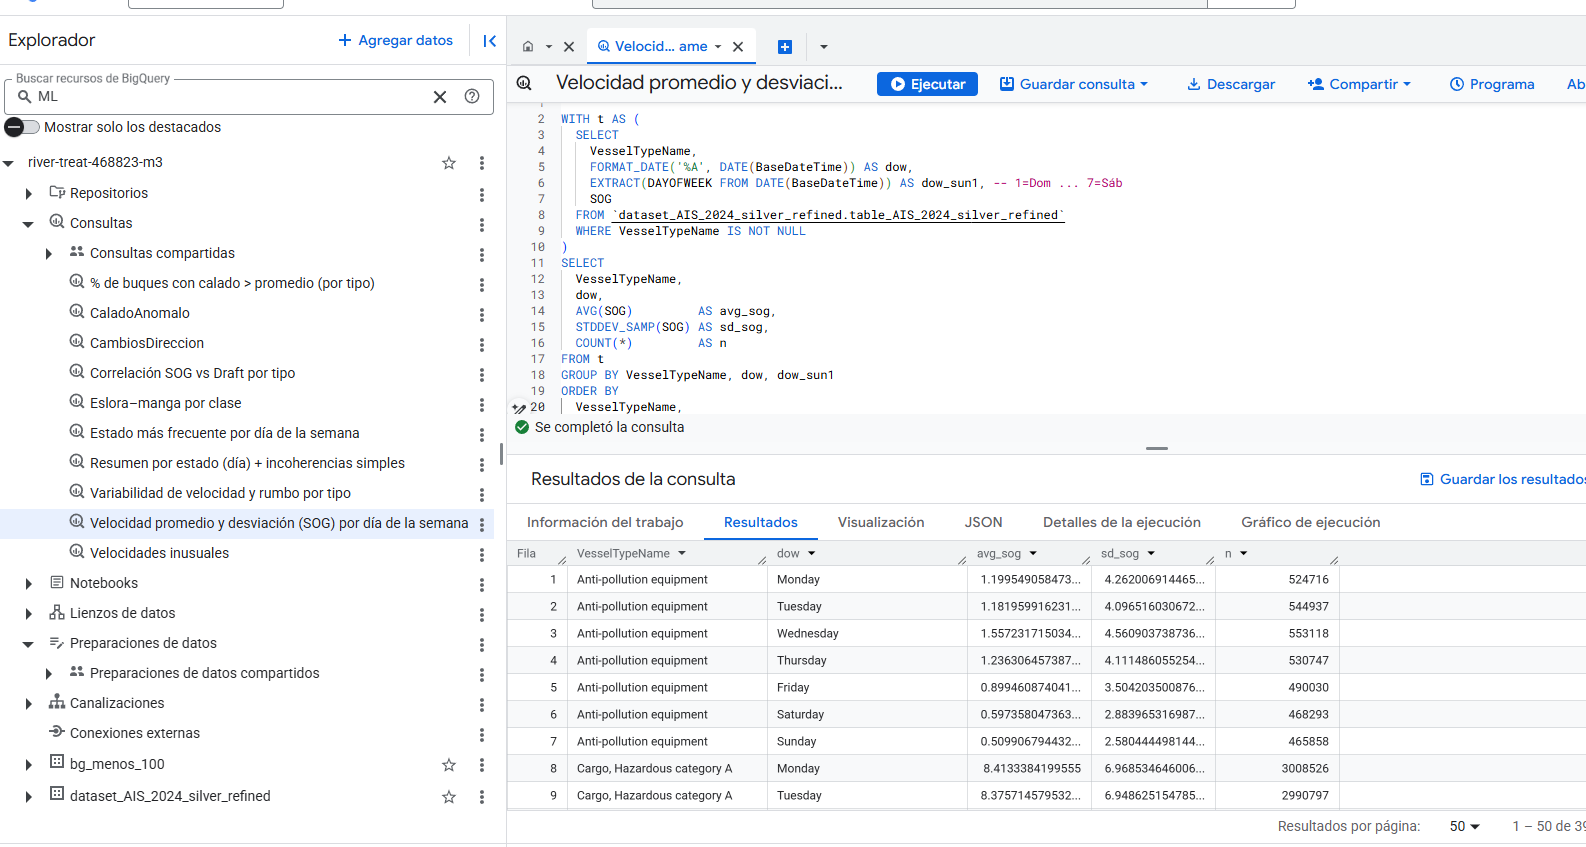
\includegraphics[width=0.6\linewidth]{figures/QuerysBQ.png}
  \caption{Pruebas y validaciones de \textit{queries} en BigQuery (comprobación de periodos, filtros y métricas).}
  \label{fig:queries-bq}
\end{figure}

\begin{figure}[htbp]
  \centering
  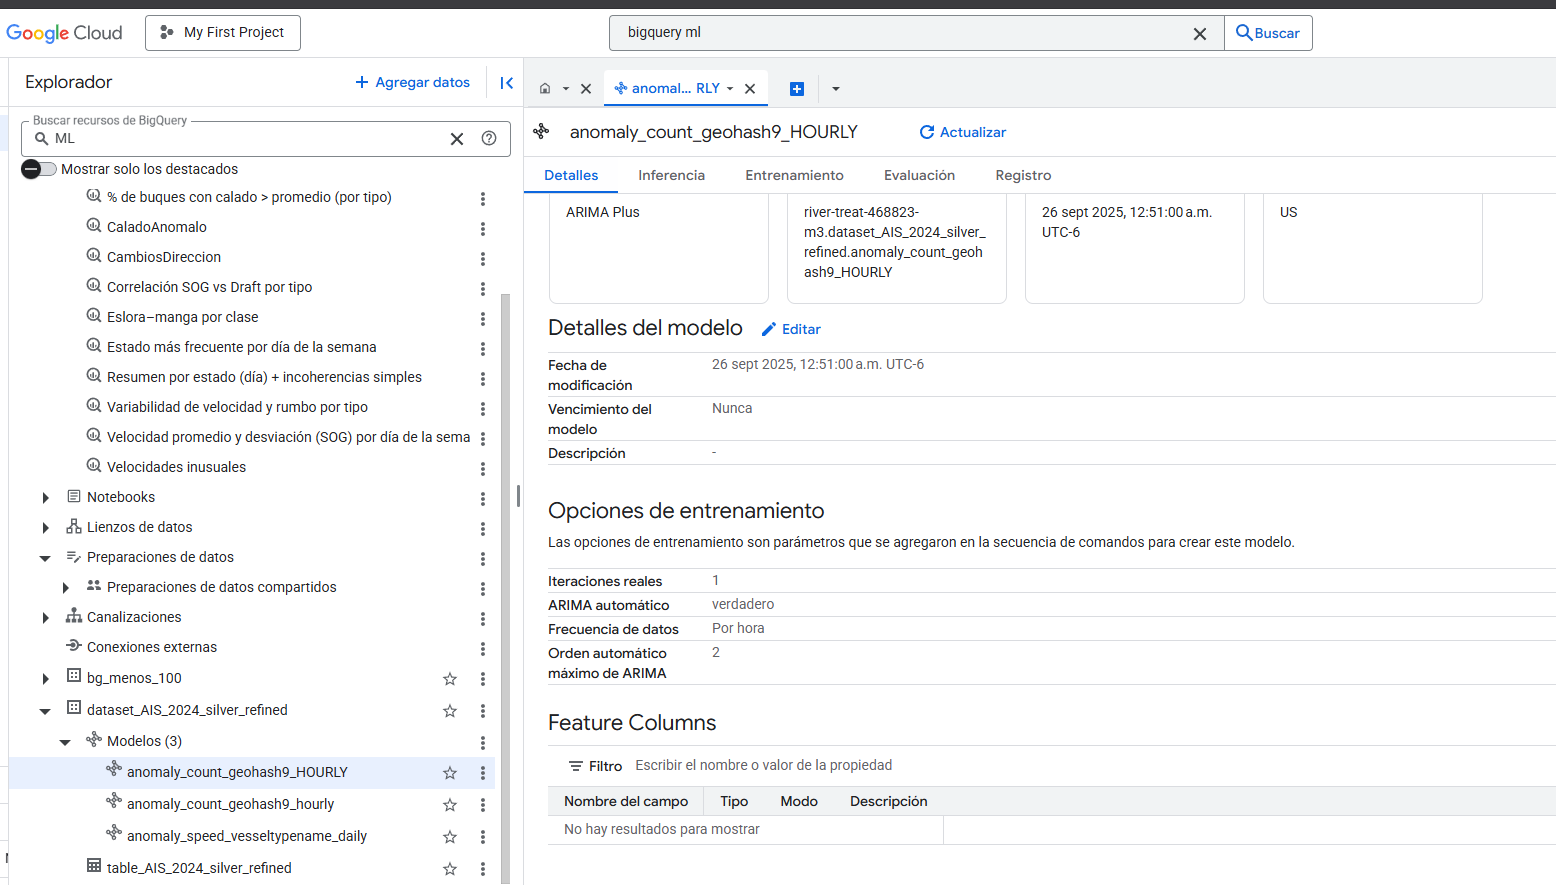
\includegraphics[width=0.6\linewidth]{figures/ModelosBQ.png}
  \caption{Verificación de entrenamiento/evaluación de modelos en BigQuery y revisión de resultados.}
  \label{fig:modelos-bq}
\end{figure}
%%%%%%%%%%%%%%%%%%%%%%%%%%%%%%%%%%%%%%%%%%%%%%%%%%%%%%%%%%%%%%%%%%%%%%%%%%%%%%%%%%%%%%%%%%%%%%%%%%%%%%%%%%%%%%%%%%%%%%%%%%%%%%%%%%%%%%%%%%%%%%%%%%%%%%%%%%%%%%%%%%%%%%%%%%%%%%%%%%%%%%%%%%%%%%
\section{Resultados y conclusiones}

Se desarrolló un \textit{dashboard} interactivo que ejecuta las consultas validadas sobre los datos AIS y expone una superficie de entrenamiento y predicción basada en \texttt{BigQuery ML (ARIMA\_PLUS)}. El tablero permite explorar coherencias/incoherencias de los mensajes, correlaciones geométricas y de desempeño, así como detectar comportamientos anómalos por serie y periodo. En conjunto, las visualizaciones y la interfaz de ML habilitan un flujo completo: (i) análisis exploratorio y verificación de datos; (ii) entrenamiento del modelo; (iii) evaluación de anomalías y revisión de resultados.
\newpage
\paragraph{Exploración y métricas.}
Los módulos de exploración incluyen: (a) correlación \emph{Eslora–Manga} por clase de buque, útil para detectar casos geométricamente atípicos; (b) \emph{Calado anómalo} a partir de \textit{z-score} por embarcación; (c) \emph{Cambios de dirección} por encima de un umbral angular configurable, con soporte de filtro geográfico; y (d) variabilidad de velocidad y rumbo, más vistas complementarias (velocidad por día de semana, estados de navegación frecuentes). Estas vistas, además de presentar tablas paginadas, ofrecen gráficas de barras y de dispersión que facilitan identificar extremos y patrones.

\paragraph{Entrenamiento y detección de anomalías.}
La ventana de ML permite seleccionar métrica (\textit{count} o \textit{speed}), frecuencia (\texttt{HOURLY/DAILY}) e identificador de serie (\texttt{geohash9}, \texttt{VesselTypeName} o \texttt{MMSI}), ejecutar el entrenamiento y, posteriormente, lanzar la detección de anomalías sobre el rango de evaluación. Los resultados se listan en tabla y se visualizan con gráficos (barras por serie y dispersión temporal), con control del umbral de probabilidad para ajustar sensibilidad/especificidad. Este flujo fue verificado con consultas de prueba previas, asegurando que los \textit{queries} de entrenamiento y predicción devuelven esquemas y valores consistentes antes de su integración final.

\begin{figure}[H]
  \centering
  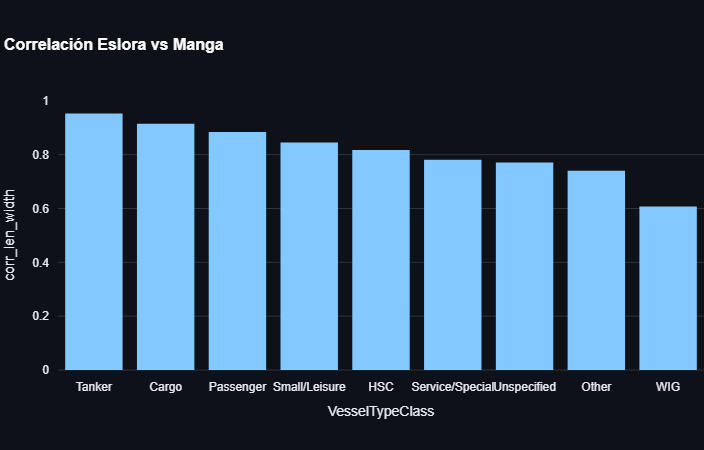
\includegraphics[width=0.6\linewidth]{figures/EsloraManga.png}
  \caption{Correlación Eslora–Manga por clase de buque.}
  \label{fig:eslora-manga}
\end{figure}

\begin{figure}[H]
  \centering
  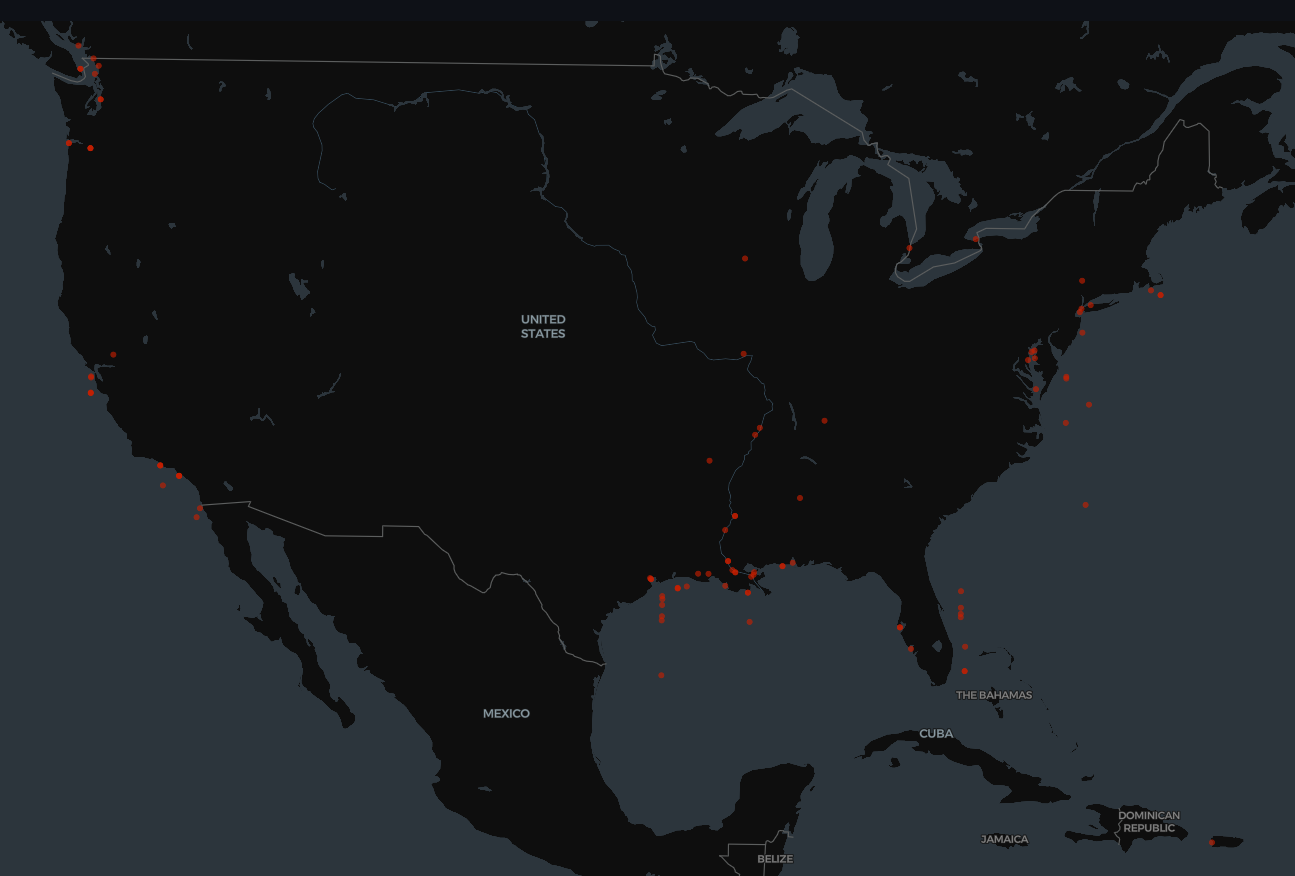
\includegraphics[width=0.6\linewidth]{figures/CambiosDireccion.png}
  \caption{Eventos de cambio de dirección por encima de un umbral angular.}
  \label{fig:cambios-direccion}
\end{figure}

\begin{figure}[H]
  \centering
  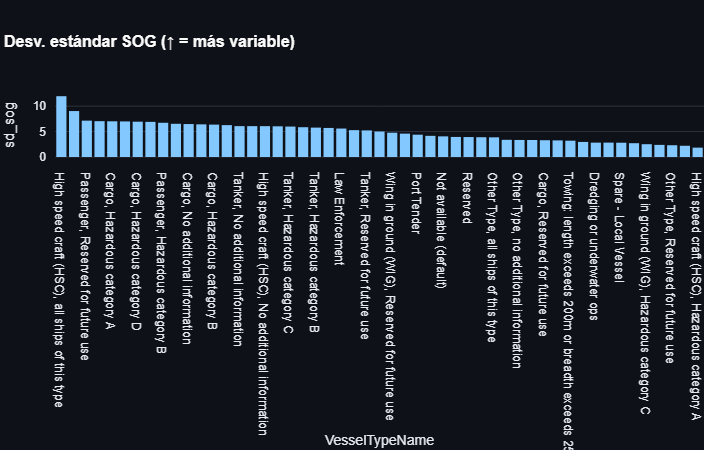
\includegraphics[width=0.6\linewidth]{figures/DesvVelRumbo.png}
  \caption{Variabilidad de velocidad y rumbo por tipo de buque.}
  \label{fig:desv-vel-rumbo}
\end{figure}

\begin{figure}[H]
  \centering
  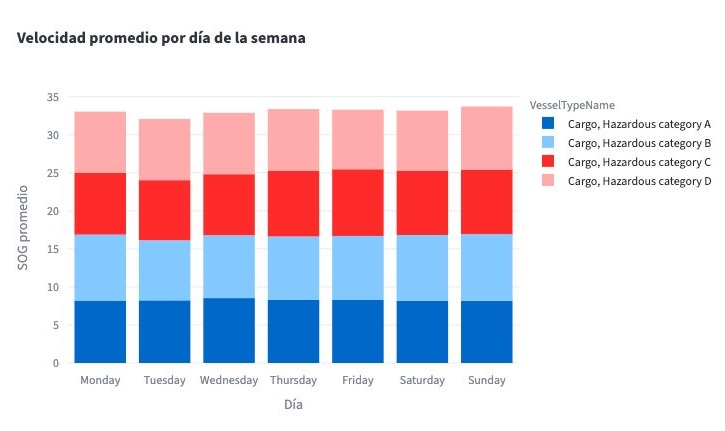
\includegraphics[width=0.6\linewidth]{figures/VelPromDiaria.jpeg}
  \caption{Velocidad promedio por día de la semana (barras apiladas por tipo de buque).}
  \label{fig:vel-prom-dia}
\end{figure}

\begin{figure}[H]
  \centering
  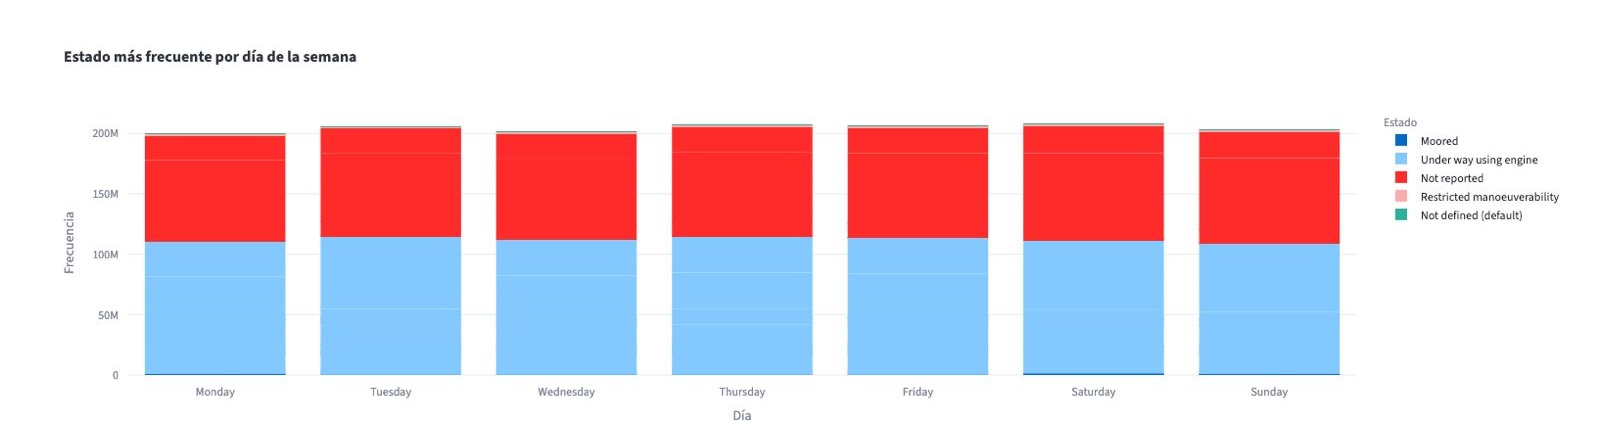
\includegraphics[width=0.6\linewidth]{figures/EstadosDiaSemana.jpeg}
  \caption{Estado de navegación más frecuente por día de la semana.}
  \label{fig:estado-dia-semana}
\end{figure}

\begin{figure}[H]
  \centering
  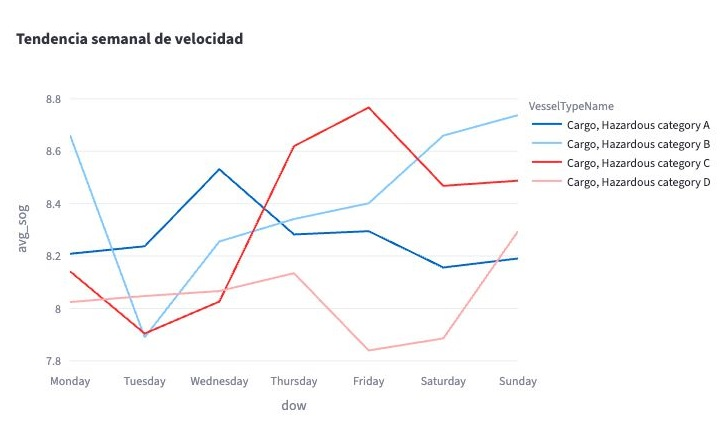
\includegraphics[width=0.6\linewidth]{figures/TendenciaSemanalVel.jpeg}
  \caption{Tendencia semanal de velocidad por tipo de buque.}
  \label{fig:tendencia-semanal-vel}
\end{figure}

\begin{figure}[H]
  \centering
  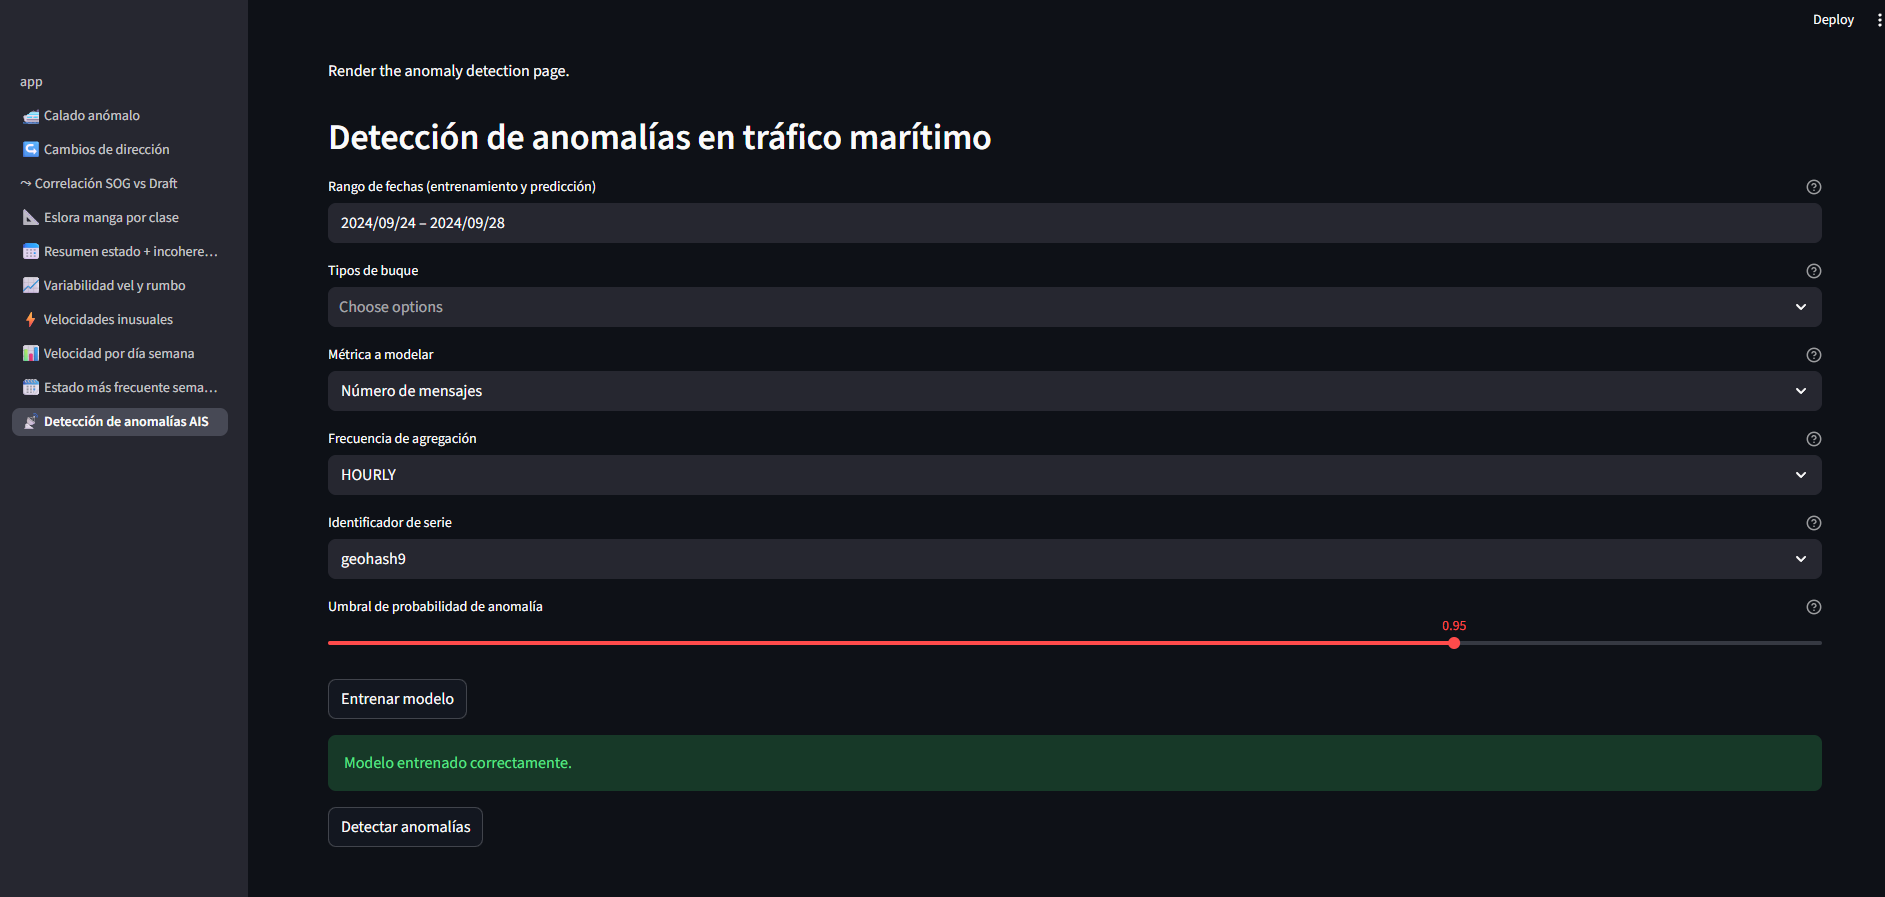
\includegraphics[width=0.6\linewidth]{figures/Entrenamiento.png}
  \caption{Ventana de entrenamiento y detección de anomalías con \texttt{BigQuery ML}.}
  \label{fig:entrenamiento}
\end{figure}

\subsection{Conclusión general}

Se implementó un flujo \emph{end-to-end} en Google Cloud que transforma datos masivos AIS en análisis operables y detección de anomalías: ingesta y preparación (GCE $\rightarrow$ GCS $\rightarrow$ DataProc/Spark), explotación analítica y de ML en BigQuery, y un \textit{dashboard} en Streamlit con ventana de entrenamiento y predicción mediante \texttt{BigQuery ML (ARIMA\_PLUS)}.

\paragraph{Aportaciones principales.}
\begin{itemize}
  \item \textbf{Pipeline reproducible y escalable} con capas \textit{raw/curated}, particionado temporal e idempotencia, optimizado para costos y tiempos de consulta.
  \item \textbf{Analítica descriptiva accionable} (patrones semanales de velocidad y estados, coherencias geométricas y de desempeño) para priorizar zonas, buques y ventanas temporales.
  \item \textbf{Detección de anomalías temporal} basada en series (ARIMA\_PLUS) con umbral configurable e integración directa en la interfaz para análisis y depuración de resultados.
\end{itemize}

\paragraph{Lecciones y limitaciones.}
\begin{itemize}
  \item La \textbf{calidad y cobertura} del AIS condicionan los hallazgos; se requieren normalizaciones y validaciones previas en SQL.
  \item La versión actual opera en \textit{batch} con disparadores manuales/programados y no incluye tiempo real.
  \item \textbf{Control de costos (GCS/BigQuery):} el volumen y la granularidad elevan costos de almacenamiento y consulta; se mitigarían con presupuestos/alertas de gasto.
\end{itemize}


%%%%%%%%%%%%%%%%%%%%%%%%%%%%%%%%%%%%%%%%%%%%%%%%%%%%%%%%%%%%%%%%%%%%%%%%%%%%%%%%%%%%%%%%%%%%%%%%%%%%%%%%%%%%%%%%%%%%%%%%%%%%%%%%%%%%%%%%%%%%%%%%%%%%%%%%%%%%%%%%%%%%%%%%%%%%%%%%%%%%%%%%%%%%%%
%%%%%%%%%%%%%%%%%%%%%%%%%%%%%%%%%%%%%%%%%%%%%%%%%%%%%%%%%%%%%%%%%%%%%%%%%%%%%%%%%%%%%%%%%%%%%%%%%%%%%%%%%%%%%%%%%%%%%%%%%%%%%%%%%%%%%%%%%%%%%%%%%%%%%%%%%%%%%%%%%%%%%%%%%%%%%%%%%%%%%%%%%%%%%%
\section{Código utilizado} 
\subsection{Link al repositorio con código fuente y salidas correspondientes}
\url{https://github.com/enriquegomeztagle/MCD-BigData-SmartMaritimeTrafficMonitoring-FinalProject}
%%%%%%%%%%%%%%%%%%%%%%%%%%%%%%%%%%%%%%%%%%%%%%%%%%%%%%%%%%%%%%%%%%%%%%%%%%%%%%%%%%%%%%%%%%%%%%%%%%%%%%%%%%%%%%%%%%%%%%%%%%%%%%%%%%%%%%%%%%%%%%%%%%%%%%%%%%%%%%%%%%%%%%%%%%%%%%%%%%%%%%%%%%%%%%
%%%%%%%%%%%%%%%%%%%%%%%%%%%%%%%%%%%%%%%%%%%%%%%%%%%%%%%%%%%%%%%%%%%%%%%%%%%%%%%%%%%%%%%%%%%%%%%%%%%%%%%%%%%%%%%%%%%%%%%%%%%%%%%%%%%%%%%%%%%%%%%%%%%%%%%%%%%%%%%%%%%%%%%%%%%%%%%%%%%%%%%%%%%%%%
\end{document}
%%%%%%%%%%%%%%%%%%%%%%%%%%%%%%%%%%%%%%%%%%%%%%%%%%%%%%%%%%%%%%%%%%%%%%%%%%%%%%%%%%%%%%%%%%%%%%%%%%%%%%%%%%%%%%%%%%%%%%%%%%%%%%%%%%%%%%%%%%%%%%%%%%%%%%%%%%%%%%%%%%%%%%%%%%%%%%%%%%%%%%%%%%%%%%
